\vspace{10pt}

{\centering\subsection*{白水:朗读是一种好的阅读方式吗?}}

\addcontentsline{toc}{subsection}{白水:朗读是一种好的阅读方式吗?}

\renewcommand{\leftmark}{白水:朗读是一种好的阅读方式吗?}

\begin{figure}[htbp]

\centering

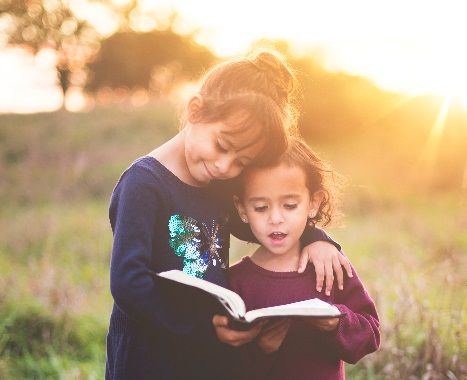
\includegraphics[width = .5\textwidth]{./ch/v1.jpg}

\end{figure}

各位家长朋友们,大家好。



这一周我们非常感谢吴才俊妈妈的视频分享。


关于朗读这个主题分享,我们想与大家一起探讨。



首先,朗读是阅读的一种方式。



对于低年级的孩子,朗读是一种有效的值得鼓励的阅读方式。朗读是一种发声表演,是一种输出,所以朗读可以让孩子更加的专注,而且可以加强记忆力。孩子可以从朗读中体会到文字的情景,体会到声音的旋律。



其次,朗读适合经典的文本,适合反复练习。



因为朗读相比于无声阅读来说,速度还是比较慢,所以比较适合经典的文本。另外,朗读也适合对一篇文章进行反复练习,从而达到最佳的效果。朗读一遍可能掌握不住文字的含义,语音的节奏,所以需要反复调整,最好能有一个观众给与反馈。



再者,朗读适合与无声阅读配合,尤其进入高年级后,要增加无声阅读的比重。仅仅朗读,可能会造成只能默读文字,而使得阅读速度比较慢,甚至产生阅读障碍。



最后,除了文字书籍,生活是最好的书籍。多接触大自然,感受和留意大自然的细节,从而获得真实的、多元的、丰富的感受和第一体验。如果从来没听过知鸟的鸣叫,没看到过水滴在荷叶上的场景,即便文字再优美,也很难写出真实感人的作品。



谢谢大家。

\vspace{10pt}

作者:白水

朗读:白水

发布:2021年4月10日

















                



\vspace{10pt}

\hline

